%This is the second chapter of the dissertation

%The following command starts your chapter. If you want different titles used in your ToC and at the top of the page throughout the chapter, you can specify those values here. Since Columbia doesn't want extra information in the headers and footers, the "Top of Page Title" value won't actually appear.
\pagestyle{plain}

\chapter[Controlling and Monitoring performance of large scale Silicon Photonic devices][Top of Page Title]{Controlling and Monitoring performance of large scale Silicon Photonic devices}

\textit{\textbf{Abstract - } In this chapter, we develop scalable solutions for controlling optical properties and in-line power monitoring of silicon photonic device. The first part of the chapter concerns with model development of the thermo-optic effect of integrated heaters. Building on the analytical models, we present a control scheme based on pulse-width modulation (PWM) signals to demonstrate a DAC-less resonance control in MRR. A study in the required PWM frequency is presented and experimentally measured to achieve a minimal ripples operation in the optical domain.}

\textit{The second part of the chapter is focused on doped heater elements, and their associated photo-conductance (PC) effect. Measuring the change of the heater conductance, enables to utilize this heater design for both controlling and optical power monitoring purposes. We show this mechanisms when doped heaters are integrated in micro-ring and Mach-Zehnder devices. The PC effect is experimentally characterized for the steady state and the transient response and compact models for the PC current are developed.}

\section{Introduction}

The Silicon Photonic platform provides a wide ranges of elements to support a variety of applications in high-speed optical communications. From coherent generation \cite{novack2018silicon} and switching \cite{vujicic2017software} to direct detection \cite{aoki2017low} links with total aggregated bandwidths in the order of Tbps. Theses designs consist of tenth to hundreds of integrated elements, and recent studies showed that these links can achieve an overall energy consumption below 2pJ/bit \cite{bahadori2016energy,bahadori2017energy} which is a highly desirable metric system performance. Achieving these highly efficient performances in practice requires that each element in the system is operated at its optimal conditions to overcome fabrication variations \cite{chrostowski2014impact} and compensated for thermal sensitivity \cite{padmaraju2014resolving}. 

As in electronics, where transistors are biased to a specific operational point, a similar principle holds with integrated photonic devices. For example, due to the narrow-band nature of the MRRs, when used as receivers or transmitter, their resonance must biased to the desired WDM channel \cite{bogaerts2012silicon}. Mach-Zehnder based modulators are biased to the linear point of the transfer function \cite{li2013any} and in a cascaded configurations when used as filters \cite{Guan_1xN,horst2013cascaded} or switches \cite{chen2016low} they are biased to the desired routing configuration. \textbf{can add more citations from the thermal paper}

The most common technique for biasing SiP elements is by means of precise control the local temperature of waveguide's section. Integrated micro-heating structures are fabricated using either metallic traces on top of the waveguide \textbf{atabaki2010optimization} or by doping the waveguide \cite{harris2014efficient}. When applying ohmic power in these heaters, the optical behavior is changed due to the high the thermo-optic coefficient in Silicon material \cite{komma2012thermo}. Effectively, by changing the index of refraction with thermal control, we manipulate the phase of the optical carrier in the thermal region []. 

Designs based on external heaters must take into account the fact that heat diffusion is not instantaneous -- it takes time for the heat to propagate from the heater to the waveguide. Moreover, the heat might reach the waveguide at different strengths and different delays.  The optical operation of the photonic device depends, therefore, on the frequencies of the electrical excitation signal applied to the heater. Understanding this transient thermal response is crucial to finely adjust and efficiently counter-balance the thermal noise that impacts the response of silicon photonic devices. 


%Current discussion of transient thermal response is reduced to experimental considerations, specifically a posteriori characterizations of rise and fall times (the time required for the temperature of the waveguide to evolve from 10\% to 90\% and 90\% to 10\% of its asymptotic values, respectively), while the stationary thermal response is straightforward to model accurately \cite{wang2017fast}.  Observing the importance of thermal stabilization in the total power budget of a photonic link \cite{bahadori2017energy}, we conclude that the understanding of thermal effects in silicon photonics platform deserves careful study 

The first goal of this chapter is to provide a comprehensive analysis and models for the thermo-optic effects in the SiP platform. Then we study how thermal variations affecting temperature-dependent devices can be adequately rectified with digitally driven signals. In particular, we look at thermal tuning using pulse width modulation (PWM) signals generated by relatively simple digital logic \cite{matsuura2017accelerating, zecevic2015integrated, aguinaldo2014wideband}. 

Our motivation for investigating PWM control is due to the fact that as the number of active SiP devices increases and reach hundred to thousands elements in integrated photonic applications []. The use of traditional digital-to-analog converters (DACs) in heterogeneous integration can be problematic to support such a high number of elements. As an alternative, a single FPGA with large number of I/Os can supports such systems. Additionally, the use of PWM control paradigm, the total power consumption of the driving circuitry can be further reduced comparing to constant voltage solutions \cite{zecevic2015integrated}. 

The second goal of this chapter is utilizing photo-conductance (PC) effect in silicon photonic doped thermo-optic phase-shifter (waveguide-doped heaters) \cite{Harris_heater}. As the optical signal (continuous or modulated) propagates through this heater design, the interaction between photons and impurities in the doped silicon generates free electrical carriers \cite{jayatilleka2019photoconductive}. As a result, the conductance of the heater is increasing proportionally with the optical power. We characterize the PC effect in MRR and MZI based designs, and develop a compact model for the photo-conductance current. 

From a system prospective, this functionality is highly desirable since it enables utilizing doped heaters as both controlling and \textit{in-line} power monitoring elements. Furthermore, it can greatly reduce design complexity which does not require tapping the signal for monitoring purposes[], reduce the total footprint area, and the number of I/O in closed-loop solutions [].

\section{Integrated Heater and Waveguide System}

By applying an electrical control to the integrated heater element, we locally change the temperature of a waveguide section. The temperature change affects the effective index of refraction of the waveguide, and as a result adjusting the phase of the propagating optical signal. The is described by the following equation:

\begin{equation}
\label{CH3_eq1}
     \Delta n_\text{eff} \approx dn_\text{eff}/dT \times \Delta T.
\end{equation}

where the thermo-optic sensitivity of a silicon waveguide surounded by a silica waveguide $dn_\text{eff}/dT$ =  2.1$\times$10$^{-4}$ K$^{-1}$. 

A schematic of the waveguide and a heater system is shown in Fig. \ref{CH3_fig2}(a). A strip waveguide with a micro-heater situated at a distance $d$. By applying a voltage to the heater, $V(t)$, the corresponded current is, $I(t)$, and the total dissipated ohmic power is $P(t)$ = $V(t)\times I(t)$ that causes the waveguide temperature to rise ($\Delta T_H$). To develop an expression

We are interested in expressing the temperature rise $\Delta T_H$ as a function of the applied voltage $V(t)$. We first note that would the resistance of the heater $R$ stay constant, the power dissipated would be strictly a quadratic function of the voltage as $I(t)$ = $V(t)/R$ and thus $P(t)$ = $V^2 (t)/R$. However, as the heater temperature increases, the resistivity of the heater increases according to $R$ = $R_\text{linear} (1 + \alpha_H \Delta T_H$) where $\alpha_H$ is the temperature coefficient of the resistance of the heater ($\alpha_H \sim 3\times 10^{-3}-8\times 10^{-3}$ K$^{-1}$ for most metals). The increased resistivity leads in turn to a decrease of the current and dissipated ohmic power. The self-heating situation of the heater finally regulates itself at a steady sate of temperature and supplied current. We assume that the self-heating of heater is instantaneous, i.e. the resistivity of the heater instantaneously changes with a change in the applied voltage. As further detailed in Appendix I, the temperature of heater linearly depends on the dissipated ohmic power where the proportionality coefficient is considered to be constant over time. The temperature of heater then follows the voltage of heater according to
%
\begin{equation}\label{CH3_eq2}
\Delta T_H = \frac{1}{2\alpha_H}\left(-1+\sqrt{1 + K_v V^2 (t)}\right)
\end{equation}
%
where $K_v$ represents the thermal nonlinearity of the ohmic resistance. The result of such self-heating phenomenon is a nonlinear DC voltage-current characteristic of the resistive heater given by
%
\begin{equation}\label{CH3_eq3}
I(t) = \frac{V(t)}{R_\text{linear}}\times \frac{2}{1+\sqrt{1 + K_v V^2 (t)}} .
\end{equation}
%
Note that if $\alpha_H \rightarrow 0$ then $K_v \rightarrow 0$, and Eq. (\ref{eq1}) and (\ref{eq2}) reduce to the simple forms for a linear resistance. 
Fig. \ref{fig2}(b) shows an example of experimentally measured V-I data points (blue circles) along with an expected linear V-I curve (dashed red line). By fitting Eq. (\ref{eq2}) to the measured data points, we find out that with parameters $R_\text{linear}$ = 161 $\Omega$ and $K_v$ = 0.6 V$^{-2}$, the model matches the measurements quite well. Fig. \ref{fig2}(c) schematically depicts the heat distribution after the self-heating of heater is reached.







\begin{figure}[t]
\begin{center}
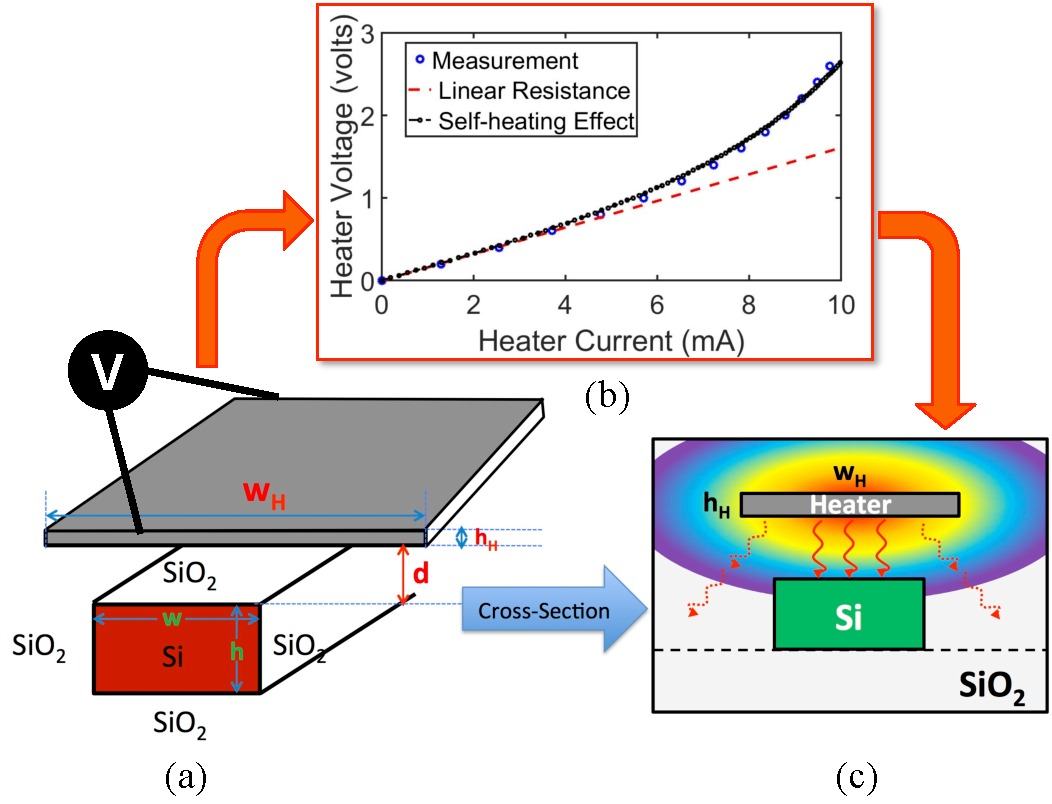
\includegraphics[width=8.5cm]{Chapter2/CH3_fig2.pdf}
\caption{(a) Structure of strip waveguide with a metallic heater situated at a distance $d$ above it. (b) V-I characteristic of the resistive heater. The nonlinear behavior is observed. (c) Schematic of heat generation at the heater and its distribution in the cladding. Dimensions are not necessarily to scale.}
\label{CH3_fig2}
\end{center}
\vspace{-0.65cm}
\end{figure}





- high capacity at low energy consumptiion

--> Phase control
--> Thermal control --> carrier injection and depletion 
--> different types of heater
--> thermal control in Mach-Zehnder vs ring 
--> response time and steady state

\section{Thermal control with pulse-width modulation}

along with a digital feedback loop for thermal control requires a large number of electrical I/O connections. Monitoring the optical operation with PWM signals has the potential to control each device with a single digital control line \cite{zecevic2015integrated, aguinaldo2014wideband}.  The main issue is to identify the frequency at which these PWM signals must be generated to obtain a stable thermal response, hence ensuring consistent optical operation. 


In the first step of our analysis we review related work (Section II) and present a preliminary analysis of the temperature sensitivity of waveguides (Section III). We then introduce an approximate analytic modeling framework for heater structures commonly used in silicon photonics platform, with an emphasis on metallic heaters. In particular, we remark that the thermal response is fundamentally governed by the heat diffusion equation. We also derive a set of expressions to describe the nonlinearity of the V-I curve of heaters, which leads us to estimates of the transient thermal response of the heater-waveguide system. We leverage this framework to analyze the thermal bandwidth of classical heater-waveguide systems (Section IV). Our analyses show that the 3dB thermal bandwidth is linearly proportional to the thermal diffusivity of the cladding material \cite{atabaki2010optimization}. To the best of our knowledge, this is the first time such a frequency model for thermal response of silicon photonic devices is proposed to characterize the trade-off between thermal bandwidth and thermo-optic efficiency. We validate our modeling framework against Finite Element Method simulations (Section V).


In the second step of our analysis we leverage our analytic framework to examine thermal rectification with a pulse width modulation (PWM) drive scheme (Section VI). In particular, we derive the relationship between the duty cycle and the required frequency of PWM excitation to obtain desired temperature conditions. These analytic conclusions are examined against experimental measurements (Section VII). Again, to the best of our knowledge, this is the first comprehensive study of PWM signaling for thermal monitoring of silicon photonic devices. 



\section{Photo-conductance effect in doped heaters}

By using the asterisk to start a new section, I keep the section from appearing in the table of contents.
If you want your sections to be numbered and to appear in the table of contents, remove the asterisk.
